\documentclass[11pt,a4paper,fleqn]{scrartcl}

\usepackage[utf8]{inputenc}
\usepackage[T1]{fontenc}
\usepackage[colorlinks=true, citecolor=blue, linkcolor=blue, filecolor=blue,urlcolor=blue]{hyperref}
\hypersetup{
     colorlinks   = true,
     citecolor    = gray
}
\usepackage{wrapfig}

\usepackage{caption}
\captionsetup{format=plain, indent=5pt, font=footnotesize, labelfont=bf}

\setkomafont{disposition}{\scshape\bfseries}

\usepackage{amsmath}
\usepackage{amssymb}
\usepackage{amsfonts}
\usepackage{bbm}
\usepackage{mathtools}
% \usepackage{epsfig}
% \usepackage{grffile}
%\usepackage{times}
%\usepackage{babel}
\usepackage{tikz}
\usepackage{paralist}
\usepackage{color}
\usepackage[top=3cm, bottom=2.5cm, left=2.5cm, right=3cm]{geometry}
%\setlength{\mathindent}{1ex}

% PGF
\usepackage{pgfplots}
\usepackage{pgf}
\usepackage{siunitx}
\usepackage{xfrac}
\usepackage{calculator}
\usepackage{calculus}
\usepackage{eurosym}
\usepackage{booktabs}
%\sisetup{per-mode=fraction,%
%	fraction-function=\sfrac}

%\newcommand{\eur}[1]{\EUR{#1}\si{\per\kilo\meter}}
\pgfplotsset{
  compat=newest,
  every axis/.append style={small, minor tick num=3}
}

%\usepackage[backend=biber,style=alphabetic,url=false,doi=false]{biblatex}
%\addbibresource{sheet01_biber.bib}
% \addbibresource{/home/coroa/papers/refs.bib}

\newcommand{\id}{\mathbbm{1}}
\newcommand{\NN}{{\mathbbm{N}}}
\newcommand{\ZZ}{{\mathbbm{Z}}}
\newcommand{\RR}{{\mathbbm{R}}}
\newcommand{\CC}{{\mathbbm{C}}}
\renewcommand{\vec}[1]{{\boldsymbol{#1}}}

\renewcommand{\i}{\mathrm{i}}

\newcommand{\expect}[1]{\langle\,#1\,\rangle}
\newcommand{\e}[1]{\ensuremath{\,\mathrm{#1}}}

\renewcommand{\O}{\mc{O}}
\newcommand{\veps}{\varepsilon}
\newcommand{\ud}[1]{\textup{d}#1\,}

\newcommand{\unclear}[1]{\color{green}#1}
\newcommand{\problem}[1]{\color{red}#1}
\newcommand{\rd}[1]{\num[round-mode=places,round-precision=1]{#1}}

%\DeclareSIUnit{\euro}{\EUR}
\DeclareSIUnit{\dollar}{\$}
\newcommand{\eur}{\text{\EUR{}}}

\usepackage{palatino}
\usepackage{mathpazo}
\setlength\parindent{0pt}
\usepackage{xcolor}
\usepackage{framed}
\definecolor{shadecolor}{rgb}{.9,.9,.9}

%=====================================================================
%=====================================================================
\begin{document}

\begin{flushright}
 \textbf{Energy System Modelling }\\
 {\small Karlsruhe Institute of Technology}\\
 {\small Institute for Automation and Applied Informatics}\\
 {\small Summer Term 2020}\\
\end{flushright}

 
 \vspace{-0.5em}
 \hrulefill
 \vspace{0.3em}

\begin{center}
 \textbf{\textsc{\Large Tutorial III: Storage Optimisation}}\\
 \small Will be worked on in the exercise session on Friday, 19 June 2020.\\[1.5em]
\end{center}

\vspace{-0.5em}
\hrulefill
\vspace{0.8em}

%=============== ======================================================
\paragraph{Problem III.1 (analytical) -- storage optimisation without losses}~\\
%=====================================================================

\begin{wrapfigure}[11]{r}{0pt}
 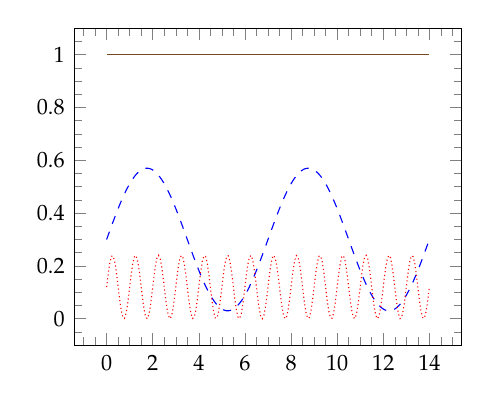
\begin{tikzpicture}
  \begin{axis}[
    domain=0:14, no markers, samples=200
    % xlabel = $x$, ylabel = $f(x)$
   ]
   \addplot+[dashed] {0.3 * (1 + 0.9 * sin(deg(2*pi*x/7)))}; \label{figref:w}
   \addplot+[densely dotted] {0.12*(1 + sin(deg(2*pi*x))}; \label{figref:s}
   \addplot+[solid] {1}; \label{figref:l}
  \end{axis}
 \end{tikzpicture}
 \caption{daily and multi-week variations of wind and solar power generation
  \(g^{N}_{w}(t)\)
  \autoref{figref:w} and \(g^{S}_{s}(t)\)
  \autoref{figref:s}, and a constant load (all in per-unit) \(L(t)\)
  \autoref{figref:l}.}
 \label{fig:variations}
\end{wrapfigure}

Imagine a two-node Germany. The South can install solar panels with a capacity factor $c_s$ to cover its load $L^S$, while the North uses wind turbines that have a capacity factor $c_w$
to feed their load $L^N$. Figure \ref{fig:variations} shows approximations to the daily and multi-week variations of per-unit wind and solar power generation \(G^{N}_{w}(t)\) and \(G^{S}_{s}(t)\) and a constant load \(L^{N/S}(t)\):

\vspace{-0.5em}

\begin{align*}
 g_{w}^N(t) & = c_w(1+A_w \sin \omega_w t), \\
 g_{s}^S(t) & = c_s(1+A_s \sin \omega_s t), \\
 L^{N/S}(t) & = A_{l}^{N/S}.
\end{align*}

The capacity factors and constants are

\begin{align*}
 A_{l}^{N} & = 20 \si{\giga\watt}, & A_{l}^{S} & = 30 \si{\giga\watt},                                         \\
 c_w    & = 0.3,                & A_w     & = 0.9,                & \omega_w & = \frac{2\pi}{7 \text{d}}, \\
 c_s    & = 0.12,               & A_s     & = 1.0,                & \omega_s & = \frac{2\pi}{1 \text{d}}.
\end{align*}

For now, assume no power exchange between the regions and that the stores are lossless.

\begin{enumerate}[(a)]
 % (a)
 \item How much wind capacity $G^{N}_{w}$ must be installed in the North and solar capacity $G_s^S$ in the South so that on average generation matches demand?

       % (b)
 \item For a system to work, generation must match demand not on average but at each location and each point in time. Storages are one way of ensuring this constraint with variable renewable generation. What is the amount of store and dispatch power capacity $G_{st,store}=\max(-\Delta(t))$ and $G_{st,dispatch} = \max \Delta(t)$ the storage units must have in the North and in the South to account for the mismatch $\Delta(t)=L(t)-G\cdot g(t)$?
\newpage
       % (c)
 \item What is the amount of energy capacity $E_{st}$ one needs for either storage in the North and in the South? The energy capacity is given by

       \begin{equation*}
        E_{st} = \max_t e_{st}(t) = \max_t \int_{0}^{t} -\Delta(t') \;\mathrm{d}t'
       \end{equation*}

       % (d)
 \item Should they choose hydrogen or battery storage? And how much would it cost them with the prices in Table 1? Is the South or the North paying more for their energy? Disregard losses!

% (e)
 \item What do you imagine would change if you considered the storage losses given in Table 1 in your results (a)-(d)?

\end{enumerate}
Now we lift the restriction against transmission and allow the two regions to bridge their 500 km separation with a transmission line.

\begin{enumerate}[(f)]
 % (f)
 \item  Estimate the cost-optimal technology mix by assuming wind energy in the North is only stored in the North and solar energy in the South is likewise only stored in the South! What would happen if you dropped that assumption?
\end{enumerate}

\begin{table}[h]
 \centering
 \label{tab:prices}
 \begin{tabular}{@{}lrrrrr@{}}
  \toprule
                             & \eur / kW & \eur / kWkm & \eur / kWh & $\eta_{store}$ & $\eta_{dispatch}$ \\ \midrule
  Battery                    & 300         & & 200          & 0.9            & 0.9               \\
  Hydrogen                   & 750         & & 10           & 0.75           & 0.58              \\
  Solar                      & 600         & &              &                &                   \\
  Wind                       & 1200        & &              &                &                   \\
  Transmission line &          & 0.4 &              &                &                   \\ \bottomrule
 \end{tabular}
 \caption{Investment costs of renewable energy infrastructure.}
\end{table}

\newpage
%=============== ======================================================
\paragraph{Problem III.2 (programming) -- storage optimization with PyPSA and losses}~\\
%=====================================================================

Python for Power System Analysis (PyPSA) is a free software toolbox for optimising modern power systems that include features such as variable wind and solar generation, storage units, etc\.. Use the toolbox to extend on your findings in Problem III.1.

To get started, you should have a look at the minimal LOPF example\footnote{\url{https://www.pypsa.org/examples/minimal_example_lopf.html}}, understand  the components documentation\footnote{\url{https://pypsa.org/doc/components.html}} of PyPSA as well as the underlying objective function and constraints in the LOPF documentation\footnote{\url{https://pypsa.org/doc/optimal_power_flow.html\#linear-optimal-power-flow}}.

\begin{enumerate}[(a)]
 \item Build a network in PyPSA with the two buses North and South and attach the load at each bus and attach the wind and solar generators with availability according to $$g^{N}_{w}(t) = c_w(1+A_w\sin \omega_w t)$$ $$g^{S}_{s}(t) = c_s(1+A_s\sin \omega_s t)$$ for a year and with \texttt{p\_nom\_extendable=True}. 
 \item Attach extendable storage units at the North and the South. The storage units have to be modelled as a \texttt{H2-bus} (a bus with \texttt{carrier='H2'}) linked to the \texttt{AC-bus} North via a \texttt{Link} where \texttt{p\_nom\_extendable=True} with the \texttt{capital\_cost} of the power capacity and an also extendable \texttt{Store} with the \texttt{capital\_cost} of the energy capacity, for instance. The losses can be set on the links as \texttt{efficiency}.
 \item Run an investment optimization by calling the \texttt{lopf} function.
 \item How do your results \texttt{objective} and \texttt{{generators,stores,links}.p\_nom\_opt} compare with the results of III.1(d) in terms of the total system costs and the capacities of the generators, stores and links?
 \item Now again lift the restriction against transmission and allow North and South to bridge their 500 km separation by adding a transmission line to the network. How does the cost optimal technology mix change compared to III.1(f)?
 \item Replace the approximated availability time-series of the wind and the solar generators with more realistic data provided in \texttt{availability.csv} computed from reanalysis weather data and re-run the linear optimal power flow. Compare the results! Explain the differences by looking at the cumulative variations relative to the mean of the availability time-series!
\end{enumerate}
\end{document}
